\documentclass[12pt,a4paper]{scrartcl}
\usepackage[utf8]{inputenc}
\usepackage{csquotes}
\usepackage[ngerman]{babel}
\usepackage{amsmath}
\usepackage{amsfonts}
\usepackage{amssymb}
\usepackage{graphicx}
\usepackage{float}
\usepackage[backend=biber]{biblatex}
\addbibresource{./sources.bib}
\author{Leon Bentrup}
\title{NSA}
\subtitle{Globale Überwaching und Demokratie?}
\begin{document}
\maketitle
\tableofcontents
\newpage
\KOMAoptions{parskip=full}

\section{Vorwort}
Dass Geheimdienste Telefongespräche und Internetverkehr überwachen, hatte ich eigentlich nie bezweifelt. Was das wirklich bedeutet, das wurde mir aber erst vor zwei Jahren bewusst.

Als im Juni 2013 auf einmal eine ganze Ladung an Informationen über geheime Projekte des amerikanischen Geheimdienstes NSA in den Medien auftauchten, als man langsam Begriff, dass es sich dabei um etwas richtig Großes handelt, da spürte ich das ungute Gefühl, dass auch bei meinen Recherchen zu dieser GFS immer wieder auftauchte.

Es fühlt sich an, als könnte man den Schlag in die Magengrube der Freiheit spüren, den die totale Überwachung jedes Menschen der Welt darstellt.

Was im Nachhinein auch völlig logisch ist, mich aber trotzdem beunruhigt, ist die Normalität, die innerhalb der Geheimdienste herrscht. Man muss sich klar machen: Analyst, die Berufsbezeichnung für die „modernen Spione“, die die abgefangenen Daten auswerten, ist ein ganz normaler Job. Analysten wechseln Arbeitgeber und haben LinkedIn-Profile mit Lebensläufen.

Manche Dokumente zeigen Geheimdienste eher als Unternehmen, statt als geheime Organisation: Es gibt Newsletter mit „Wusstest du schon?”-Artikeln, die einen über die Geschichte des ECHELON-Programms aufklären, für das Anwenden neuer Spionage-Techniken bekommen Mitarbeiter „Skillz-Points“. In anderen Worten: Die Digitalisierung der Welt hat „Spion” zu einem Bürojob gemacht.

\section{Edward Snowden}
\begin{figure}
\centering

\includegraphics[width=0.4\textwidth]{images/snowden.jpg}
\caption{Edward Snowden bei seinem Interview mit Greenwald}
\end{figure}
Edward Snowden ist die zentrale Persönlichkeit der Enthüllungen. Nach langjähriger Arbeit in verschiedenen Einrichtungen der amerikanischen Regierung. Er sammelte eigenständig Millionen von Beweisen für geheime Programme der NSA und anderen Geheimdiensten, die er dann durch die Medien an die Öffentlichkeit brachte.

\subsection{Lebenslauf}
Edward Snowden wurde am 21. Juni 1983 geboren.
Da beide Eltern für die Regierung arbeiten, ist es für ihn „normal“, das gleiche zu tun.
Nach seiner Schulzeit tritt er 2004 der U.S.-Army bei, mit dem Ziel, in Irak zu kämpfen. Als er nach 3 Monaten bei der Armee einen Trainingsunfall hatte, verließ er sie wieder.
Er arbeitete danach für einige nicht-geheime Einrichtungen der Regierung, bis er 2006, beim Besuch einer Jobmesse von der CIA rekrutiert wurde, wo er unter anderem bei einem internationalen Treffen 2008 in Genf eigesetzt wurde.
\cite{wiki_snowden}

2009 wechselte er zu DELL, er kümmerte sich um die Computersysteme von Regierungskunden, darunter auch Systeme der NSA und CIA. Sein Einkommen in dieser Position betrug etwa 200~000\$ im Jahr.
Schon dort bekam er Einsicht in einige streng geheime Operationen der NSA und sammelte schon einige Dokumente als Beweiß.

Seinen entgültigen Beschluss, die Handlungen der NSA und anderer Geheimdienste an die öffentlichkeit zu bringen, fasste er 2013. In einem Interview sagte Snowden, dass der 12. März 2013 der ausschlaggebend für seine Entscheidung gewesen sei. Dort wurde der Director of National Intelligence (nationaler Geheimdienstdirektor) der USA zur Überwachung von Amerikanern befragt, und log die Mitglieder des Kongress an, obwohl er unter Eid stand.

Daraufhin gibt Snwoden seinen Job bei DELL auf und wechselte zur Dienstleistungsfirma Booz Allen Hamilton, die Personal für die NSA zur Verfügung stellte. Er war im Geheimdienst offiziell als Systemadministrator tätig, und hatte somit uneingeschränkten Zugriff auf alle Akten des Geheimdienstes. Snowden sagte, dass zu seinen Aufgaben aber auch das Überprüfen und Angreifen feindlicher Computersysteme zählte. Seine Position nannte er „Systems Analyst”

\subsection{Enthüllungen}

\begin{figure}[H]
\centering
\begin{tabular}{lr}
Australien & 15~000 Dokumente \\
Vereinigtes Köngreich & 58~000 Dokumente \\
Department of Defense & 960~000 Dokumente \\
National Security Agency & 1~700~000 Dokumente \\
& \textbf{ca. 2~700~000 Dokumente}
\end{tabular}
\caption{Zahl der von Snowden gesammelten Dokumente}
\end{figure}

Auch wenn Snowden wollte, dass die geheimen Operationen der NSA an die Öffentlichkeit geraten, war er nicht generell gegen Überwachung. Nur solle Überwachung gezielt und auf Verdacht stattfinden, und nicht so massenhaft, wie die NSA es betreibt. 

Da er also wichtige Operationen der Geheimdienste, zum Beispiel die Überwachung von bekannten Terrororganisationen, nicht gefährden wollte, musste er beim Veröffentlichen der gesammelten Dokumente vorsichtig sein. Er sichtete zunächst selbst alles und sortierte Teile aus, die nichts mit der von ihm kritisierten Massenüberwachung zu tun hatten.

Außerdem veröffentlichte er die Dokumente nicht selbst, sondern übergab sie der Filmemacherin Laura Poitras und dem Journalisten Glenn Greenwald. Sie sollten die Dokumente dann über die Medien an die Öffentlichkeit bringen.

\subsubsection{Laura Poitras}
Laura Poitras, geboren am 2. Februar 1964 in Boston, ist Produzentin und Filmemacherin. Sie arbeitet seit 2005 an einer Filmreihe über die Welt nach dem 11. September 2001. Nachdem sie den ersten Film der Trilogie veröffentlicht hat, wird sie regelmäßig an der amerikanischen Grenze kontrolliert und befragt. Aus diesem Grund zieht sie nach Berlin um, als sie mit ihrem Film „Citizenfour” beginnt. Sie befürchtet, dass ihr Filmmaterial beschlagnahmt wird.\cite{praxisfilms}

\subsubsection{Glenn Greenwald}
Der amerikanische Journalist Glenn Greenwald, der am 6. März 1967 in New York geboren wurde, ist die zweite Person, die Snowden kontaktierte. Er studierte Philosophie und Rechtswissenschaften.\cite{wiki_greenwald} Von 1996 bis 2005 arbeitete er in einer eigenen Anwaltskanzlei, die sich auf Verfassungs- und Bürgerrechte (von US-Bürgern) spezialisierte.\cite{unclaimed_response}

In seinen Blog „Unclaimed Territory“ schrieb Greenwald bis 2007 unter anderem über frühere Affären der NSA, bis er später zum Online-Magazin „salon.com“ und schließlich im Juni 2012 zur britischen Tageszeitung „The Guardian” wechselte. Im Guardian veröffentlichte Greenwald auch den ersten Artikel über das Snowden-Material.\cite{wiki_greenwald}

2014 gründete er zusammen mit Laura Poitras die Nachrichtenseite „The Intercept“.\cite{intercept_about}

\section{Überwachung}
% Allgemeines

\subsection{XKeyscore}


\subsection{Five Eyes}
Die NSA ging mit einigen anderen Geheimdiensten Partnerschaften ein. Darunter zählte auch der Deutsche Bundesnachrichtendienst. Die „wichtigsten” Partner waren allerdings:
\begin{itemize}
\item \textbf{GCHQ}, Government Communications Headquarters, \emph{Vereinigtes Königreich}
\item \textbf{DSD}, Defense Signals Directorate, \emph{Australien}
\item \textbf{CSEC}, Communications Security Establishment Canada, \emph{Kanada}
\item \textbf{GCSB}, Government Communications Security Bureau, \emph{Neuseeland}
\end{itemize}

Zusammen mit der NSA selbst, nennen sich diese Geheimdienste die „Five Eyes”.
Das Abkommen zwischen den Five Eyes beinhaltete eine „No-Spy-Vereinbarung”, die Partner haben sich also gegenseitig nicht abgehört, es gab allerdings auch Außnahmen von dieser Regel. Außerdem teilten die Bündnispartner sämtliche gesammelten Daten und entwickelte Technologien. So hatten alle Geheimdienste der Five Eyes Zugriff auf NSA-Programme wie XKeyscore oder PRISM.

\subsubsection{Umgehung von Beschränkungen durch die Verfassung}
Das Five Eyes-Bündnis wurde auch genutzt um verfassungsrechtliche Beschränkungen zu umgehen. So darf die NSA zum Beispiel nach der 4. Ergänzung zur Unabhängikeitserklärung der Vereinigten Staaten keinen amerikanischen Staatsbürger abhören. Der britische Geheimdienst GCHQ, der dies natürlich darf, hört dann für die NSA deren Ziel ab und gibt die gesammelten Daten an sie weiter.

\subsection{TEMPORA}
Zu den Technologien, die die Five Eyes untereinander weitergeben, gehört auch das Projekt des britischen GCHQ, „Tempora“. Hinter Tempora verbirgt sich eine Instanz des amerikanischen XKeyscore-Systems.

Tempora ist das mit Abstand größte XKeyscore-System. Mehr als 1000 Server an mehr als 3 Standorten ermöglichen das Mitschneiden der Kommunikation über Glasfaserkabel.

Großbritanniens geografische Lage ist für dieses Unternehmen sehr vorteilhaft. In Europa liegt es am nächsten zur amerikanischen Ostküste. Deshalb verlaufen fast alle Untersee-Glasfaserkabel zwischen Europa und Amerika durch Großbritannien. Über diese Glasfaserkabel werden alle Internet- und Telefonverbindungen zwischen den Kontinenten übertragen.

Der GCHQ verschafft sich durch Abkommen mit den Betreibern der Internetknoten Zugang zu diesen Kabeln, und ist somit in der Lage 480 GBit/s (Das 48 Millionenfache der durchschnittlichen Internetgeschwindigkeit in Deutschland\cite{statista_internet}) an Daten in Echtzeit zu sammeln, zu sortieren und zu speichern. Die gesamte Kommunikation, mit Inhalt der Verbindungen werden für 3 Werktage gespeichert. Deshalb nennt der GCHQ das System auch einen „Internet Buffer”, einen Zwischenspeicher für das Internet, der die globale Kommunikation „verlangsamt” und im Nachhinein durchsuchbar macht. Die Metadaten, also Sender, Empfänger, deren Aufenthaltsort und Informationen über deren Endgeräte, Betreff und Zeitpunkt der Nachrichten werden für 30 Tage gespeichert.

\section{Verhältnis zu Deutschland}
Die NSA nannte Deutschland einen „Partner dritter Klasse“. Das bedeutet, dass Deutschland, obwohl es ein Abkommen mit der NSA geschlossen hat, abgehört wird. Die NSA sammelt ungefähr so viele Datensätze über Deutschland, wie sie auch über China und Russland sammelt. (Siehe Abbildung~\ref{fig:boundless_informant})

% Boundless Informant
\begin{figure}[H]
\centering
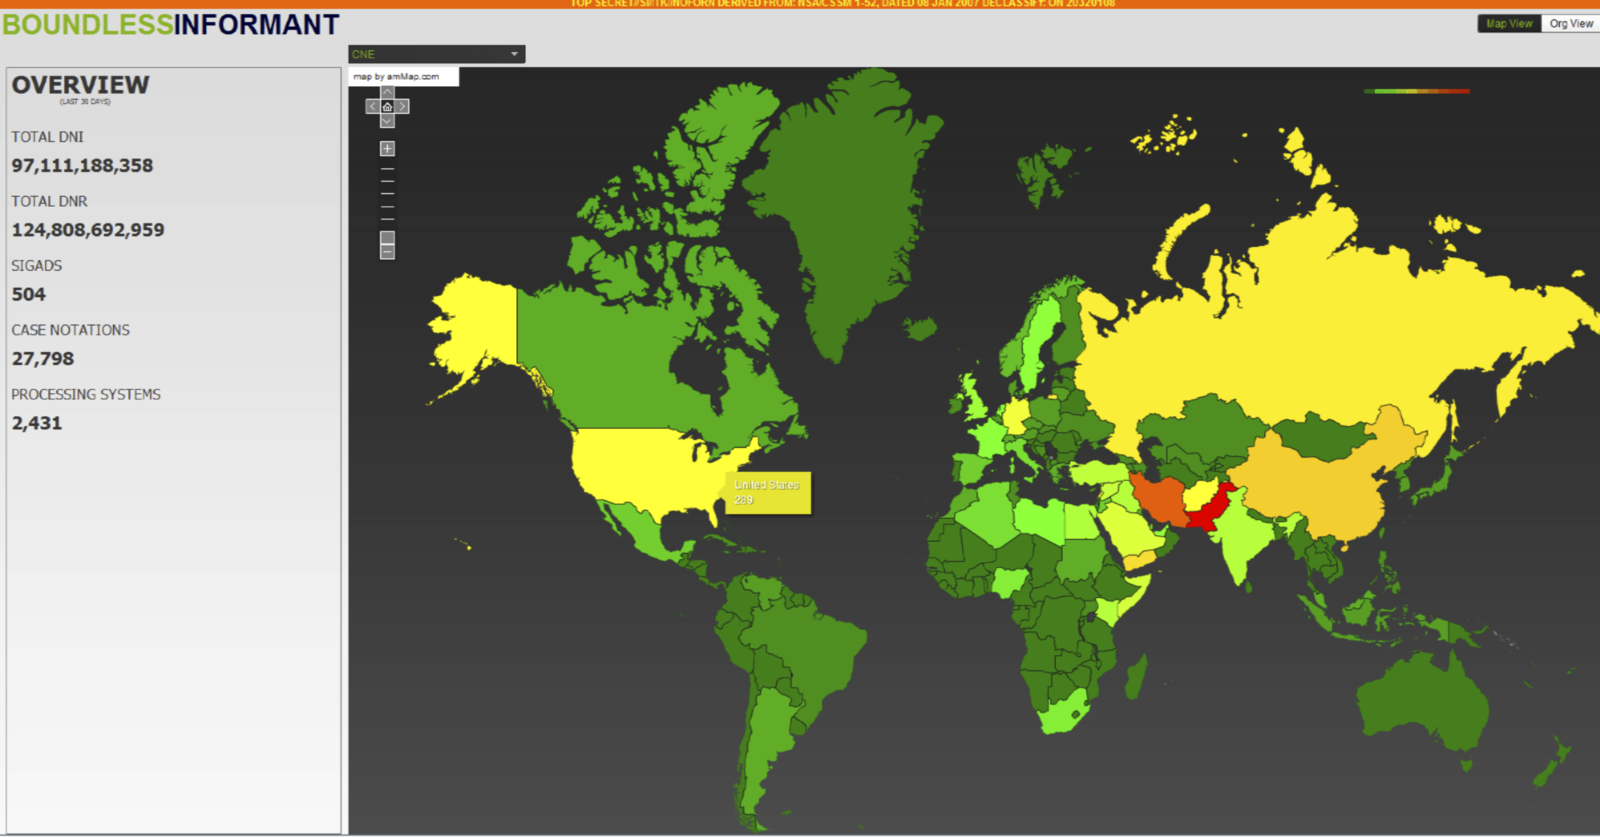
\includegraphics[width=\textwidth]{images/bi.png}
\caption{Übersicht über von der NSA gesammelten Daten nach Land (Boundless Informant)}
\label{fig:boundless_informant}
\end{figure}

\subsection{Partnerschaft mit der NSA}
Die Rahmenbedingungen, die die Partnerschaft zwischen Bundesnachrichtendienst, Verfassungsschutz und der NSA kennzeichnen, sind in einem Dokument namens „Terms of Reference“ festgehalten.

Die NSA übergibt dem BND das XKeyscore-System, welches dieser dann auf eigenen Servern einsetzen kann. Außerdem darf der BND das System an das Bundesamt für Verfassungsschutz weitergeben. Im Gegenzug gibt Deutschland so viele Daten wie möglich an die NSA weiter, falls diese für deren Ermittlungen relevant sein könnten.

\subsection{Operation Eikonal}
Die umstrittenste Operation des BND, die bei den Untersuchungen des NSA-Ausschusses im Bundestag bekannt wurde, ist die „Operation Eikonal“.

Neben Großbritannien ist auch Deutschland ein wichtiger Standort des Internet-Glasfasernetzes in Europa. In Frankfurt am Main befindet sich der DE-CIX, der am Datendurchsatz gemessen, der größte Internetknoten der Welt ist.

Zu einigen der vielen Glasfaserleitungen im DE-CIX verschaffte sich der BND Zugang. Er installierte so genannte „Taps“, die den Datenverkehr duplizieren, die Daten werden also zum einen an den Empfänger weitergeleitet, zusätzlich dazu, wird aber eine Kopie der Daten ausgeleitet. Über eine Standleitung wird dann ein Teil der so abgefangenen Daten in den BND-Standort in Pullach weitergeleitet, dort kann er analysiert werden.

Ob dieses Verfahren rechtmäßig ist, wurde schon von Anfang an bezweifelt, auch von Mitarbeitern des BND selbst. Deshalb wurde die Operation Eikonal angeblich 2008 eingestellt. Vor dem NSA-Untersuchungsausschuss sagte ein BND-Mitarbeiter:

\begin{quotation}
Eikonal beinhaltete selektive Erfassung von Ausland-Ausland-Transitverkehr. Zeit nicht vergessen: Afghanistan, Terror-Aufklärung. Da wurden selektiert Daten erfasst und automatisiert weitergeleitet. Genaueres nur nicht-öffentlich. Wir machen die Methodik ja immer noch.
\end{quotation}

Es ist also fraglich, ob Eikonal 2008 wirklich eingestellt wurde.
\section{Geheimdienste in Deutschland}

\subsection{MAD}

\subsection{BfV}

\subsection{BND}

\section{Fazit}

\newpage
\printbibliography
\newpage

Hiermit erkläre ich, dass ich die vorliegende Arbeit selbstständig und ohne fremde Hilfe verfasst und keine anderen Hilfsmittel als angegeben verwendet habe. Insbesondere versichere ich, dass ich alle wörtlichen und sinngemäßen Übernahmen aus anderen Werken als solche kenntlich gemacht habe.
\vspace{2cm}
\hrule
\end{document}
